% Options for packages loaded elsewhere
\PassOptionsToPackage{unicode}{hyperref}
\PassOptionsToPackage{hyphens}{url}
%
\documentclass[
]{article}
\usepackage{amsmath,amssymb}
\usepackage{iftex}
\ifPDFTeX
  \usepackage[T1]{fontenc}
  \usepackage[utf8]{inputenc}
  \usepackage{textcomp} % provide euro and other symbols
\else % if luatex or xetex
  \usepackage{unicode-math} % this also loads fontspec
  \defaultfontfeatures{Scale=MatchLowercase}
  \defaultfontfeatures[\rmfamily]{Ligatures=TeX,Scale=1}
\fi
\usepackage{lmodern}
\ifPDFTeX\else
  % xetex/luatex font selection
\fi
% Use upquote if available, for straight quotes in verbatim environments
\IfFileExists{upquote.sty}{\usepackage{upquote}}{}
\IfFileExists{microtype.sty}{% use microtype if available
  \usepackage[]{microtype}
  \UseMicrotypeSet[protrusion]{basicmath} % disable protrusion for tt fonts
}{}
\makeatletter
\@ifundefined{KOMAClassName}{% if non-KOMA class
  \IfFileExists{parskip.sty}{%
    \usepackage{parskip}
  }{% else
    \setlength{\parindent}{0pt}
    \setlength{\parskip}{6pt plus 2pt minus 1pt}}
}{% if KOMA class
  \KOMAoptions{parskip=half}}
\makeatother
\usepackage{xcolor}
\usepackage[margin=1in]{geometry}
\usepackage{longtable,booktabs,array}
\usepackage{calc} % for calculating minipage widths
% Correct order of tables after \paragraph or \subparagraph
\usepackage{etoolbox}
\makeatletter
\patchcmd\longtable{\par}{\if@noskipsec\mbox{}\fi\par}{}{}
\makeatother
% Allow footnotes in longtable head/foot
\IfFileExists{footnotehyper.sty}{\usepackage{footnotehyper}}{\usepackage{footnote}}
\makesavenoteenv{longtable}
\usepackage{graphicx}
\makeatletter
\def\maxwidth{\ifdim\Gin@nat@width>\linewidth\linewidth\else\Gin@nat@width\fi}
\def\maxheight{\ifdim\Gin@nat@height>\textheight\textheight\else\Gin@nat@height\fi}
\makeatother
% Scale images if necessary, so that they will not overflow the page
% margins by default, and it is still possible to overwrite the defaults
% using explicit options in \includegraphics[width, height, ...]{}
\setkeys{Gin}{width=\maxwidth,height=\maxheight,keepaspectratio}
% Set default figure placement to htbp
\makeatletter
\def\fps@figure{htbp}
\makeatother
\setlength{\emergencystretch}{3em} % prevent overfull lines
\providecommand{\tightlist}{%
  \setlength{\itemsep}{0pt}\setlength{\parskip}{0pt}}
\setcounter{secnumdepth}{5}
% definitions for citeproc citations
\NewDocumentCommand\citeproctext{}{}
\NewDocumentCommand\citeproc{mm}{%
  \begingroup\def\citeproctext{#2}\cite{#1}\endgroup}
\makeatletter
 % allow citations to break across lines
 \let\@cite@ofmt\@firstofone
 % avoid brackets around text for \cite:
 \def\@biblabel#1{}
 \def\@cite#1#2{{#1\if@tempswa , #2\fi}}
\makeatother
\newlength{\cslhangindent}
\setlength{\cslhangindent}{1.5em}
\newlength{\csllabelwidth}
\setlength{\csllabelwidth}{3em}
\newenvironment{CSLReferences}[2] % #1 hanging-indent, #2 entry-spacing
 {\begin{list}{}{%
  \setlength{\itemindent}{0pt}
  \setlength{\leftmargin}{0pt}
  \setlength{\parsep}{0pt}
  % turn on hanging indent if param 1 is 1
  \ifodd #1
   \setlength{\leftmargin}{\cslhangindent}
   \setlength{\itemindent}{-1\cslhangindent}
  \fi
  % set entry spacing
  \setlength{\itemsep}{#2\baselineskip}}}
 {\end{list}}
\usepackage{calc}
\newcommand{\CSLBlock}[1]{\hfill\break\parbox[t]{\linewidth}{\strut\ignorespaces#1\strut}}
\newcommand{\CSLLeftMargin}[1]{\parbox[t]{\csllabelwidth}{\strut#1\strut}}
\newcommand{\CSLRightInline}[1]{\parbox[t]{\linewidth - \csllabelwidth}{\strut#1\strut}}
\newcommand{\CSLIndent}[1]{\hspace{\cslhangindent}#1}
\usepackage{indentfirst}
\usepackage{sectsty}
\allsectionsfont{\centering}
\usepackage{fontspec}
\usepackage{polyglossia}
\setdefaultlanguage{english}
\setotherlanguages{russian}
\setmainfont{Times New Roman}
\newfontfamily{\cyrillicfonttt}{Times New Roman}
\usepackage{float}
\usepackage{float} \floatplacement{figure}{H}
\newcommand{\beginsupplement}{\setcounter{table}{0}
\renewcommand{\thetable}{S\arabic{table}}
\setcounter{figure}{0}
\renewcommand{\thefigure}{S\arabic{figure}}}
\usepackage{fancyhdr}
\pagestyle{fancy}
\usepackage{booktabs}
\usepackage{longtable}
\usepackage{array}
\usepackage{multirow}
\usepackage{wrapfig}
\usepackage{float}
\usepackage{colortbl}
\usepackage{pdflscape}
\usepackage{tabu}
\usepackage{threeparttable}
\usepackage{threeparttablex}
\usepackage[normalem]{ulem}
\usepackage{makecell}
\usepackage{xcolor}
\ifLuaTeX
  \usepackage{selnolig}  % disable illegal ligatures
\fi
\usepackage{bookmark}
\IfFileExists{xurl.sty}{\usepackage{xurl}}{} % add URL line breaks if available
\urlstyle{same}
\hypersetup{
  pdftitle={Guilt, shame, and anti-war action in an authoritarian country at war},
  hidelinks,
  pdfcreator={LaTeX via pandoc}}

\title{Guilt, shame, and anti-war action in an authoritarian country at war}
\author{}
\date{\vspace{-2.5em}}

\begin{document}
\maketitle

\fancyhead[LH]{GUILT, SHAME, AND ANTI-WAR ACTION}
\fancyhead[RH]{}

\vspace{10mm}
\begin{center}
Lusine Grigoryan$^{1}$, Vladimir Ponizovskiy$^{2}$, Marie Isabelle Wießflog$^{2}$, Evgeny Osin$^{3,4}$, and Brian Lickel$^{5}$
\vspace{30mm}

$^{1}$ Department of Psychology, University of York
\vspace{5mm}

$^{2}$ Department of Psychology, Ruhr University Bochum
\vspace{5mm}

$^{3}$ LINP2 Lab, Université Paris Nanterre
\vspace{5mm}

$^{4}$ Department of Psychology, HSE University
\vspace{5mm}

$^{5}$ Department of Psychological and Brain Sciences, University of Massachusetts Amherst
\vspace{40mm}

\end{center}

\noindent This is a computationally reproducible version of the final paper. The version of record was published in \emph{Political Psychology}, and is available at: \url{https://doi.org/10.1111/pops.12985}

\vspace{10mm}

\noindent We have no known conflict of interest to disclose.

\noindent All study materials, data, and code can be found on the OSF platform:

\noindent \url{https://osf.io/4pd2v/?view_only=23597fdc19424706818a72fc0df43009}

\noindent Correspondence concerning this article should be addressed to Lusine Grigoryan, University of York,

\noindent Psychology Building, Heslington, York YO10 5NA, UK. Email: \href{mailto:lusine.grigoryan@york.ac.uk}{\nolinkurl{lusine.grigoryan@york.ac.uk}}

\pagebreak

\section*{Abstract}\label{abstract}
\addcontentsline{toc}{section}{Abstract}

Feeling guilt and shame for the harm done to others by the ingroup can facilitate intergroup reconciliation. Most of the studies showing this effect are conducted in democratic countries and on historical, not current, conflicts. We investigated the role of group-based guilt and shame in collective action in an authoritarian country at war. We asked more than 1000 Russians living in Russia, in a sample representative of the country's population by gender and age, about their experiences of group-based guilt and shame regarding Russia's invasion of Ukraine and their past and future anti-war political actions. We tested whether political efficacy is necessary for experiencing group-based guilt and shame, and whether these emotions are predictive of anti-war action over and above other emotions and attitudes. Democratic values, not political efficacy, were the most robust predictor of group-based guilt and shame. Only moral shame, but not image shame or guilt predicted past and future anti-war action. Whereas attitude towards the war and moral shame predicted engagement in anti-war action (vs none), other negative dominant emotions like anger predicted the degree of this engagement. We highlight the gaps in the study of collective action and the need for more evidence from non-democratic contexts.

\vspace{5mm}

\emph{Keywords}: group-based emotions, guilt, moral shame, image shame, collective action, Russia-Ukraine war, authoritarianism

\section*{Guilt, shame, and anti-war action in an authoritarian country at war}\label{guilt-shame-and-anti-war-action-in-an-authoritarian-country-at-war}
\addcontentsline{toc}{section}{Guilt, shame, and anti-war action in an authoritarian country at war}

On February 24, 2022, Russia, the country with the biggest nuclear warhead inventory in the world, invaded the neighboring Ukraine. Although the Russia-Ukraine war started in 2014 with the occupation of Crimea, Russian officials consistently denied their involvement in the region. Eight years later, Russia openly invaded Ukraine on four fronts: North (Kyiv), North-East (Kharkiv), South-East (Donetsk and Luhansk), and South (Crimea). The official ideological narrative supporting the invasion was provided in a televised speech by Vladimir Putin preceding the invasion by mere minutes. In this speech, Putin falsely claimed that Ukraine is governed by a group of neo-Nazis who hold the population hostage and persecute the Russian speakers in the country. The announced goals of this ``special military operation'' (the use of the word ``war'' soon after will be criminalized in Russia) were the ``denazification'' and ``demilitarization'' of Ukraine.

In the first days following the invasion, thousands of Russians took to the streets to protest. However, nearly 15.000 people were detained in the first weeks following the invasion (OVD-Info, 2022) and the street protests quickly died down. New laws were introduced regularly to further suppress protest, among them the law about the ``discreditation of the Russian armed forces'', which essentially prohibited any anti-war statements or actions (Eckel, 2022). After the introduction of this law, the few remaining independent media outlets either stopped covering the war or left the country (The Moscow Times, 2022).

Against the backdrop of the reports of war crimes committed by the Russian armed forces in Ukraine and the repression of all dissent in Russia, the discussions among the well-educated Russians, many of whom left the country, often revolved around the topics of collective responsibility, guilt, and shame (e.g., Grigoryan and Ponizovskiy, 2022; Treus, 2022). As these discussions took shape, it became clear that the majority view, even among the Russian ``intelligentsia'' that opposed the war, is that feelings of guilt and shame are inappropriate or even harmful (Kynev, 2022). For example, in a series of interviews with prominent Russian intellectuals and artists, Ekaterina Gordeeva, a journalist with more than 1.5 million subscribers on YouTube, asked each of her guests whether they feel guilt or shame for what is happening in the country; with very few exceptions, the answer was ``no'' (Gordeeva, 2022). The push-back against the idea of feeling guilt or shame for what your country is doing was so strong that soon a new hashtag \#IamNotAshamed (\#МнеНеСтыдно) became popular across social media platforms.

Research on group-based guilt and shame and collective action has been predominantly carried out in Western democracies {[}with notable exception of a number of studies on the Israeli-Palestinian conflict; Roccas et al. (2006); Weiss-Klayman et al. (2020){]}. Although there is strong evidence that experiencing these emotions can motivate people to engage in collective action and support intergroup reconciliation efforts and oppose military actions by one's country (Hakim et al., 2021; Iyer et al., 2007; Lickel et al., 2011), research on preconditions for experiencing these emotions and on the power of these emotions to motivate collective action in authoritarian regimes is lacking. One could argue that when people have no control, or believe that they have no control, over the decisions of their government, feelings of guilt and shame would not arise or would not be associated with behavioral outcomes, as they are in democratic contexts, where these emotions serve the function of regulating ingroup's moral behavior. If the ingroup's behavior cannot be changed, then these emotions might lose their functionality and be downregulated. Is the sense that one has some control over the political events in their country a necessary precondition for feeling group-based guilt and shame? Are these feelings relevant in authoritarian regimes? Can they motivate behavior in such contexts? We set out to address these questions in Russia, an authoritarian country at war.

In this paper, we present the results of a large-scale, preregistered online survey of Russian population conducted in August 2022. We aim to address the following three research questions: (1) Are feelings of group-based guilt and shame conditional upon political beliefs that people can influence the actions of their governments? (2) Are guilt and shame predictive of anti-war action in an authoritarian state? (3) Are guilt and shame better predictors of anti-war action than other emotions or attitudes?

\section*{Theoretical background}\label{theoretical-background}
\addcontentsline{toc}{section}{Theoretical background}

\allsectionsfont{\raggedright}

\subsection*{Group-based guilt and shame}\label{group-based-guilt-and-shame}
\addcontentsline{toc}{subsection}{Group-based guilt and shame}

Group-based emotions are emotions elicited by actions of fellow ingroup members (Iyer and Leach, 2008). Social groups are necessary for human survival and both positive and negative group-based emotions can help regulate the behavior of group members, promoting desirable (e.g., through pride) and inhibiting undesirable (e.g., through guilt) behaviors. The function of group-based guilt and shame is to ensure good conduct of group members by signaling instances of norm violations and motivating restorative action (Lickel et al., 2011).

Although the emotions of guilt and shame share many similarities (Smith and Ellsworth, 1985) and are often experienced simultaneously (Schmader and Lickel, 2006), they also have some important differences in appraisals and motivations. The feeling of shame is likely to occur when the ingroup member's negative actions reflect poorly on the group identity itself, whereas the feeling of guilt -- when one feels collective responsibility for the negative actions of group members. As a result, shame is expected to motivate avoidant behaviors (hiding, distancing), whereas guilt is expected to motivate approach behaviors (repairing, restoring) (Lickel et al., 2011; Tangney et al., 2007).

This prediction that particular moral emotions are linked uniquely to different forms of intergroup behavior (with guilt linked to reconciliatory behavior and shame linked to avoidance) is not well supported by the empirical evidence available so far. A recent meta-analysis of group-based emotions ((Hakim et al., 2021), 101 effect sizes, 58 samples, N = 10,305) found that guilt, shame, and anger are equally predictive of support for reparations, with a strong average effect size of r = .44 and no significant differences between emotions. Furthermore, theHow can this inconsistency regarding the impact of shame on reconciliatory behaviors be explained?

The distinction between moral shame and image shame (Allpress et al., 2010; Rees et al., 2013) helps explain which elements of shame are predictive of reconciliatory behaviors and which are predictive of avoidant behaviors. This distinction is made based on different appraisals that the feeling of shame can be accompanied with: we feel moral shame when the group members' behavior violates important moral standards or values of the group, and we feel image shame when the group members' behavior tarnishes the ingroup's reputation (Rees et al., 2013). Studies that make the distinction between moral shame and image shame find that moral shame is predictive of reconciliatory behaviors on par or more strongly than guilt, whereas image shame is predictive of distancing and avoidance (Allpress et al., 2014; Allpress et al., 2010; Grigoryan and Efremova, 2017; Nooitgedagt et al., 2021; Rees et al., 2013). We therefore expect that moral shame and guilt, but not image shame, will predict a stronger intention to act against the war in Russia (H1).

\subsection*{Acknowledgement of responsibility as a precondition for experiencing guilt and shame}\label{acknowledgement-of-responsibility-as-a-precondition-for-experiencing-guilt-and-shame}
\addcontentsline{toc}{subsection}{Acknowledgement of responsibility as a precondition for experiencing guilt and shame}

Although rarely studied, the acknowledgement of collective responsibility for the ingroup's wrongdoings could be a necessary precondition for experiencing group-based guilt and shame. In a series of experiments, Cehajić-Clancy et al. (2011) showed that guilt mediates the effect of an intervention designed to increase acknowledgement of responsibility for the ingroup's wrongdoing and support for reparations. Consistent with this finding, a recent set of studies showed that beliefs of group malleability shape experiences of guilt and shame (Weiss-Klayman et al., 2020): participants who believed that groups can change and those who thought that others believe that groups can change (meta-beliefs) showed higher levels of guilt and shame.

Applying these findings to international conflicts where the ingroup is the country, we argue that experiences of group-based guilt and shame are conditional upon beliefs that citizens have control over and responsibility for their governments' decisions. This belief would form the foundation for acknowledgment of collective responsibility, which would then translate into the feelings of group-based guilt and shame and, consequently, anti-war or reconciliatory behavior. We expect that the higher the belief that citizens have control over political decisions in their country, the stronger are the feelings of guilt and shame (H2). We test this prediction by measuring different constructs that tap into the notion of political control and responsibility: political alienation (Olsen, 1969), political cynicism (Pattyn et al., 2012), democratic values (Canetti-Nisim and Beit-Hallahmi, 2007), and political responsibility.

Various definitions and operationalizations have been suggested for both political cynicism and political alienation constructs, but broadly, both capture a belief that the political process is run without input from ordinary citizens, that politics and politicians can't be trusted, and that political participation is futile (Litt, 1963; Schwartz, 1973). Both political alienation and cynicism have been shown to predict political non-participation (Adams et al., 2006; Pinkleton and Weintraub Austin, 2004). As political alienation and cynicism would indicate disengagement and dis-identification with the political process, we predict that higher levels of alienation and cynicism would predict lower levels of group-based shame and guilt. It is possible that political cynicism could be associated with anti-government attitudes and behavior, but only when operationalized as mistrust of the current government (Erber and Lau, 1990). When operationalized as apathy and withdrawal from the political process, we expect the effects of political alienation and cynicism in authoritarian contexts would be similar to those in democratic contexts.

Conversely, democratic values and the notion of political responsibility highlight the importance of political participation. Democratic values represent support for key democratic principles such as freedom of speech, minority rights, and the rule of law (Canetti-Nisim and Beit-Hallahmi, 2007), and political responsibility represents a belief that people have a responsibility to participate in the political process. Democratic values have been repeatedly shown to predict political participation (Chang, 2017; Karp and Milazzo, 2015; Oser and Hooghe, 2018). We predict that higher levels of support for democratic values and political responsibility would predict higher levels of group-based shame and guilt because both support for democratic values and political responsibility beliefs imply engagement with the political process. One could argue that the conflict between democratic values and a non-democratic political process in an authoritarian state would lead to dis-identification and political disengagement among those who strongly support democratic values. However, we believe it more likely that the disengagement of people from politics in authoritarian states is achieved (besides repressions) by a combination of making democracy seem less desirable and of corrupting the meaning of what democracy means (see the distinction between liberal and authoritarian notions of democracy, Kirsch and Welzel, 2018). We would expect that in any authoritarian state, those most motivated to change the status quo, and therefore those who would feel most negative emotions about the wrongdoings of their state, would be those who support liberal democratic values.

\subsection*{Collective action in an authoritarian state}\label{collective-action-in-an-authoritarian-state}
\addcontentsline{toc}{subsection}{Collective action in an authoritarian state}

The integrative social identity model of collective action (SIMCA) -- perhaps the most comprehensive and widely used model of collective action in psychology -- identifies three key components of collective action: perceived injustice, identity, and efficacy (van Zomeren et al., 2008). In a meta-analysis of more than 180 independent samples, van Zomeren et al. (2008) found that each of these three components uniquely predict collective action, with similar effect sizes. As the diversity of samples and issues studied grew in recent years, authors extended the model by introducing moral beliefs as a key component of the model (van Zomeren et al., 2018). The updated meta-analysis (Agostini and Zomeren, 2021) introduces the dual chamber model of collective action, which places identity and morality as two interrelated and equally fundamental motivational drivers of collective action that translate into action via perceptions or feelings of injustice and efficacy.

This meta-analysis (Agostini and Zomeren, 2021) incorporates 1.235 effects from 403 samples with a total sample size of over 120.000. Among other things, the meta-analysis looks into structural constraints on motivations for collective action. Although many limitations remain regarding diversity of samples and issues studied, and political regime or the democracy index are not included in the analysis, some variables can serve as indirect indicators of how restrictive the social context is. These include Western vs.~non-Western samples (assuming the West is on average more democratic), collectivism cultural dimension from Hofstede (assuming behavior is regulated more strongly in collectivist societies), and hierarchy -- egalitarianism cultural dimension from Schwartz (assuming more hierarchical societies are more restrictive). Keeping in mind all the limitations of such approximation, it is worth noting that the effect of morality in collective action was stable across all moderator variables, whereas the effect of identity varied considerably and was weaker in non-Western, collectivistic, and more hierarchical societies. This suggests that the content of identity, including who is defined as ``us'', what it means to be ``us'', and how politicized this identity is can vary considerably across contexts. Based on these meta-analytical findings, we would expect morality, i.e., moral shame, to be the most robust predictor of collective action in the Russian context.

This expectation is supported by other studies that looked specifically at collective action in non-democratic contexts. In a series of studies in five non-democratic states (Egypt and Turkey in 2013, Russia, Ukraine, and Hong Kong in 2014), Ayanian and colleagues (Ayanian et al., 2021; Ayanian and Tausch, 2016) show how perceptions of risk in repressive contexts can have counter-intuitive effects on willingness to participate in collective action. While perceived risk can quell collective action through increased fear, it can also spur resistance through increased outrage and heightened feelings of moral obligation. Contributing to this line of research, we will test how guilt and moral shame compare to other predictors of collective action and whether they are predictive of anti-government action in an authoritarian state over and above other emotions and attitudes (RQ1).

\allsectionsfont{\centering}

\section*{Method}\label{method}
\addcontentsline{toc}{section}{Method}

The study was approved by the ethics committee of the Psychology Department at {[}Anonymized university{]}. All study materials, including the questionnaire, data, and code, can be found on the Open Science Framework platform: \url{https://osf.io/4pd2v/?view_only=23597fdc19424706818a72fc0df43009}. The preregistration protocol is available at \url{https://aspredicted.org/SGV_SBD}. The scope of the preregistration protocol is broader than the scope of the current paper: it includes predictions regarding group-based guilt and shame, positive and negative emotions more broadly, and social identity as potential predictors of political behavior. In this manuscript, we focus on predictions regarding group-based guilt and shame and report the analyses pertaining to positive and negative emotions in the supplement. The hypotheses regarding the role of social identity (global-local identity and constructive and blind patriotism) will be the focus of a future publication.

\allsectionsfont{\raggedright}

\section*{Sample and procedure}\label{sample-and-procedure}
\addcontentsline{toc}{section}{Sample and procedure}

We collected a quota sample, representative of the Russian population by gender and age. Participants were recruited via the online crowdsourcing platform Yandex Toloka in August 2022 and completed the survey anonymously. This was the only feasible option to collect fully anonymized data in Russia, which was crucial, given that the repercussions for expressing opposition to the war can be severe. Participants received \$0.5 (30 RUB) for their participation. A total of N=1011 participants gave full informed consent to participate in the study. Thirty participants were excluded since they dropped out of the study before completion, and another eight were excluded for failing more than one out of three attention checks. The effective sample size is N=973.

The sample was balanced by gender (49.9\% women, 49.6\% men, 0.4\% non-binary or no response) and age cohort (18 to 88 years old, M=38, SD=13). About 55\% said they had lower than average income and about 51\% of the sample had a tertiary degree (BA or higher). For comparison, 63\% of 25-34 year-old Russians have tertiary education according to the latest available OECD data from 2018 (OECD, 2019). All participants were Russian citizens and 99.6\% lived in Russia\footnote{We additionally tested the robustness of our findings when excluding the participants who did not reside in Russia at the time of data collection. None of the results were affected by this exclusion.} at the time of data collection. Most (91\%) identified as ethnic Russian, 3\% as Tatar, about 1\% as Ukrainian, Chuvash, and Bashkir each, and the remaining 3\% chose the ``other'' category.

\subsection*{Measures}\label{measures}
\addcontentsline{toc}{subsection}{Measures}

The means, standard deviations, and correlations between all variables are available in Table S1 of the online supplement. Figure 1 show the distribution and correlations between group-based emotions and past and future anti-war action.

\textbf{\emph{Political beliefs.}} We used four different scales to capture participants' beliefs about political agency and the role of democracy. All items were assessed on a 7-point scale from 1 -- (\emph{absolutely disagree}) to 7 -- (\emph{absolutely agree}).

\emph{Support for democratic values} was measured with a 6-item scale from Canetti-Nisim and Beit-Hallahmi (2007). Example item: ``Every citizen has the right to take his convictions to the street if necessary'' (\(\alpha\) = 0.69; M=\texttt{r}, SD=\texttt{r}).

\emph{Political alienation} was measured with four items from Olsen (1969). Example item: ``There is not much that people like me can do to influence actions of the government'' (\(\alpha\) = 0.73).

\emph{Political cynicism} was measured with eight items from Pattyn et al. (2012). Example item: ``Politicians pretend to care more about people than they really do'' (\(\alpha\) = 0.91).

\emph{Political responsibility.} We formulated five items aimed at capturing participants' beliefs about political responsibility: ``The government will face difficulties if it tries to do something that most people in the country do not agree with'', ``Participation in political life is a responsibility of every person before themselves and their fellow countrymen'', ``If I see that the country is going in the wrong direction, it is my duty to get my voice heard by the government'', ``The citizens of Russia are accountable for the actions of their government'', ``If the majority of the citizens are against some decision made by the government, they can influence that decision'' (\(\alpha\) = 0.71).

Since the constructs of political alienation, cynicism, and responsibility are closely related and none of these scales were used in a Russian sample before, we conducted a confirmatory factor analysis (CFA) to test whether the 3-factor structure could be confirmed. The 3-factor model showed unsatisfactory fit to the data (CFI = 0.803, RMSEA = 0.128, SRMR = 0.11). An exploratory factor analysis suggested that a 4-factor model, with the political cynicism scale split in two, fits the data better. CFA confirmed this result: a model with 4 factors showed a good fit to the data (CFI = 0.947, RMSEA = 0.068, SRMR = 0.068). This modified model includes the \emph{political responsibility} factor with 5 items (M=\texttt{r}, SD=\texttt{r}), \emph{political alienation} factor with 3 items (M=\texttt{r}, SD=\texttt{r}; the item ``I believe public officials don't care much what people like me think'' was removed since it loaded on both political alienation and cynicism subscales), and two facets of political cynicism: ``\emph{politicians are bad}'' (4 items, e.g., ``Politicians are only interested in getting and maintaining power''; M=\texttt{r}, SD=\texttt{r}) and ``\emph{politics is bad}'' (4 items, e.g., ``No man can hope to stay honest once he enters politics''; M=\texttt{r}, SD=\texttt{r}).

\textbf{\emph{Positive and negative emotions.}} We measured emotions that participants experience when thinking about the war using the short version of the Positive and Negative Affect Scale {[}PANAS; Watson et al. (1988){]}. Twelve emotions (fear, joy, sadness, hope, anger, enthusiasm, disgust, pride, contempt, depression, guilt, and shame) were rated on a 5-point scale from 1 (\emph{do not experience at all}) to 5 (\emph{extremely}). If participants answered 2 or higher to the guilt and shame questions, they were shown questionnaires for group-based guilt (n=) and/or shame (n=), respectively. We took this precaution participants in earlier studies conducted in Russia complained about the double-barreled nature of items measuring group-based guilt and shame, where they felt that the questions imply that participants experience some level of guilt or shame (see Grigoryan et al. (2018); Grigoryan and Efremova (2017), for details). We tested the two-factor structure of the PANAS scale (positive and negative affect, excluding guilt and shame\footnote{We excluded guilt and shame since we planned to estimate whether group-based guilt and shame are predictive of behavior over and above other emotions. Including PANAS measures of guilt and shame into the index of negative emotions would have confounded the two measures and prevented us from addressing this question (RQ1).}) using CFA and found the fit to be unsatisfactory (CFI = 0.862, RMSEA = 0.146, SRMR = 0.08). A 3-factor structure with \emph{positive emotions} (joy, hope, enthusiasm; M=, SD=), \emph{negative dominant emotions} (anger, disgust, contempt; M=, SD=) and \emph{negative submissive emotions} (fear, sadness, depression; M=, SD=) showed a satisfactory fit to the data (CFI = 0.916, RMSEA = 0.117, SRMR = 0.066; see Mehrabian (1980) for the distinction between dominant and submissive emotions).

\textbf{\emph{Group-based guilt and shame.}} We used the measures of group-based guilt, image shame, and moral shame developed by Rees et al. (2013), Russian adaptation by Grigoryan and Efremova (2017). All items were answered on a 5-point scale from 1 (\emph{completely disagree}) to 5 (\emph{completely agree}). Guilt was measured with 3 items (e.g., ``I feel guilty for the manner in which Ukrainian people have been treated by Russians'', \(\alpha\) = 0.89), image shame with 5 items (``I feel ashamed when I realize that other countries might think of Russia negatively because of our involvement in Ukraine'', \(\alpha\) = 0.94), and moral shame with 4 items (``I feel ashamed because Russia's actions with regard to Ukraine have been immoral'', \(\alpha\) = 0.93). All missing values were replaced with zeros, since participants who didn't see the scale were the ones who reported no feelings of guilt or shame in the PANAS. With this imputation, we were able to use the whole dataset without excluding those who reported experiencing no guilt or shame. Mean values after this imputation were M=1.23 (SD=1.69) for guilt, M=1.13 (SD=1.70) for image shame, and M=1.09 (SD=1.67) for moral shame.

\textbf{\emph{Attitude towards the war}} was measured with 3 items, on a bipolar 5-point Osgood-style scale: ``The special military operation in Ukraine is\ldots{}'': bad-good, harmful-beneficial, useless-useful (\(\alpha\) = 0.9, M = 2.88, SD = 1.29).

\textbf{\emph{Anti-war actions}}. We measured \emph{past behavior} by asking how many of the eight political actions listed the participant had done to oppose the war in Ukraine (e.g., ``signing a petition'', ``participating in a demonstration'', etc.). The responses ranged from 0 to 8, with 82\% of participants reporting zero actions, M=, SD=. \emph{Behavioral intention} to participate in any political action against the war was measured with 3 items (``I want to/intend to/plan to take part in political action against the war in Ukraine''), on a 5-point scale from 1 (\emph{completely disagree}) to 5 (\emph{completely agree}) (\(\alpha\) = 0.95; 73\% of participants had a mean score of 1; M=, SD=). Finally, we asked about \emph{the probability that the person will take any political action}, from 1 (\emph{highly improbable}), 10 (\emph{(almost) certainly}) (69\% answered `1'; M=, SD=).

\allsectionsfont{\centering}

\section*{Results}\label{results}
\addcontentsline{toc}{section}{Results}

We will present the results in three parts, each addressing one of the three research questions\footnote{Question 1 in this manuscript corresponds to hypotheses 1a-1d in the preregistration protocol, question 2 -- to hypothesis 3, question 3 -- to hypothesis 5 and RQ2 from the preregistration protocol. The test of hypothesis 3 is expended beyond behavioral intentions and we additionally test the predictive power of guilt and shame for past behaviour and for probability to act in the future. The results for hypotheses 4 and 6 are reported in the SM and hypotheses 2a-2c will be the focus of a future publication.}: (1) Are feelings of group-based guilt and shame conditional upon beliefs that people can influence the actions of their governments? (2) Are guilt and shame predictive of anti-war action in an authoritarian state? (3) Are guilt and shame better predictors of anti-war action than other emotions or attitudes? Following the preregistration protocol, we use linear regression models to address these questions. However, since the outcome variables in all cases have zero-inflated distributions (see the diagonal on Fig. \ref{fig:corplots}: most participants said that they do not feel guilt or shame and did not and are not planning to take any political action against the war), we additionally tested the robustness of the findings using zero-inflated negative binomial regressions. The benefit of this approach is that it splits the variance of the dependent variable into two parts and explains each of them separately: one part of the model predicts the distinction between zero and non-zero values of the outcome (feeling an emotion or not feeling it, doing something or doing nothing, etc.) and the other part explains the value of the outcome in the non-zero part of the distribution, similar to a linear regression model. The zero-inflated part of the model predicts the likelihood of a zero value, whereas the count part of the model predicts a higher score on the outcome measures -- therefore, effects of opposite directions in these two parts of the model have the same interpretation. All additional analyses, as well as descriptive statistics for all variables (means, standard deviations, and correlations) are presented in the Supplementary Materials (SM). For all linear models tested below, we report both standardized (\(\beta\)) and unstandardized (\emph{b}) effect sizes.

\begin{figure}

{\centering 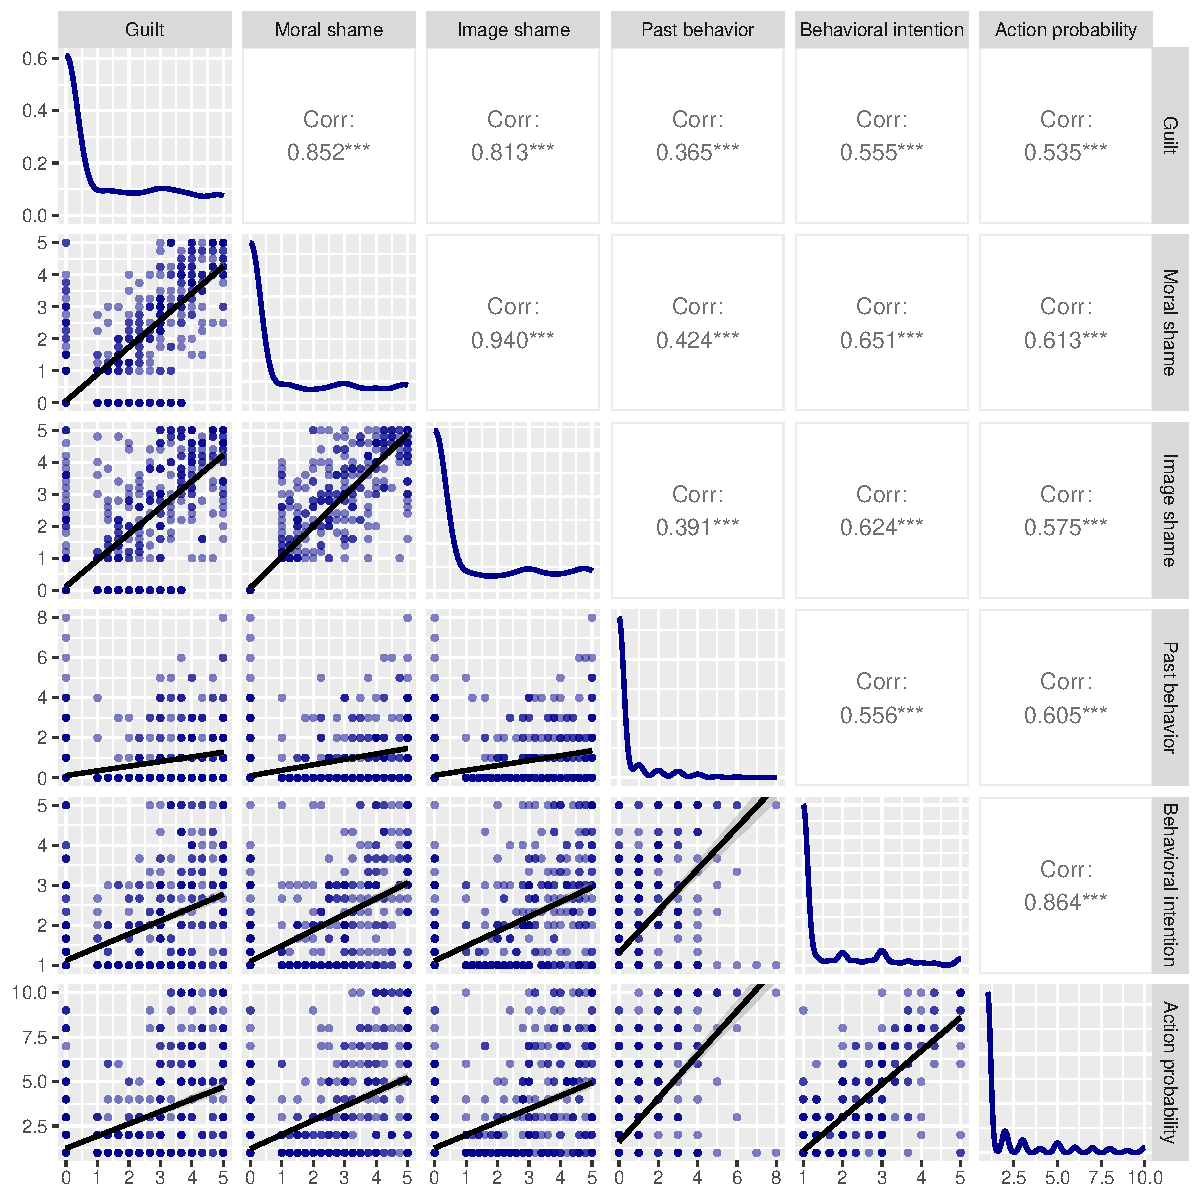
\includegraphics{corplot} 

}

\caption{Score distributions and correlations between group-based emotions and anti-war action.}\label{fig:corplots}
\end{figure}

\allsectionsfont{\raggedright}

\subsection*{Part 1. Are feelings of group-based guilt and shame conditional upon beliefs that people can influence the actions of their governments?}\label{part-1.-are-feelings-of-group-based-guilt-and-shame-conditional-upon-beliefs-that-people-can-influence-the-actions-of-their-governments}
\addcontentsline{toc}{subsection}{Part 1. Are feelings of group-based guilt and shame conditional upon beliefs that people can influence the actions of their governments?}

In a series of linear regressions, we tested whether political beliefs predict experiences of group-based shame and guilt. As Table \ref{tab:Table1} indicates, participants with stronger democratic values and those with stronger belief that politicians are bad reported stronger experiences of group-based guilt, moral shame, and image shame. The effect size of democratic values was at least twice as strong as that of political cynicism (\(\beta\) \(\approx\) .40 vs.~\(\beta\) \(\approx\) .15). Political responsibility beliefs also predicted guilt, albeit weakly. Overall, political beliefs explained 22-26\% of variance in experiences of group-based guilt and shame and the endorsement of democratic values was the main driver of these experiences. Multicollinearity was not an issue in any of the models, as all variance inflation factors (VIF) were \textless{} 3 (Vittinghoff et al. (2005) and James et al. (2013) suggest that VIF\textgreater10 indicates a serious collinearity problem). The results of the zero-inflated models (Table \ref{tab:TableS1}, SM) were essentially identical when predicting strength of the emotions. Only democratic values predicted the occurrence of emotions (zero vs.~non-zero scores).

\begin{table}[H]
\centering
\caption{\label{tab:Table1}Predicting group-based guilt and shame from political beliefs}
\centering
\fontsize{8}{10}\selectfont
\begin{tabular}[t]{lrrrrrrrrrrrr}
\toprule
\multicolumn{1}{c}{} & \multicolumn{4}{c}{Moral Shame} & \multicolumn{4}{c}{Image Shame} & \multicolumn{4}{c}{Guilt} \\
\cmidrule(l{3pt}r{3pt}){2-5} \cmidrule(l{3pt}r{3pt}){6-9} \cmidrule(l{3pt}r{3pt}){10-13}
\em{ } & \em{$\beta$} & \em{b} & \em{SE} & \em{p} & \em{$\beta$} & \em{b} & \em{SE} & \em{p} & \em{$\beta$} & \em{b} & \em{SE} & \em{p}\\
\midrule
Intercept & 0 & -2.89 & 0.32 & <.001 & 0 & -2.85 & 0.34 & <.001 & 0 & -2.93 & 0.34 & <.001\\
Democratic Values & 0.41 & 0.64 & 0.05 & <.001 & 0.4 & 0.64 & 0.05 & <.001 & 0.41 & 0.65 & 0.05 & <.001\\
Political Cynicism (politicians) & 0.18 & 0.2 & 0.05 & <.001 & 0.16 & 0.18 & 0.05 & <.001 & 0.09 & 0.1 & 0.05 & .039\\
Political Cynicism (politics) & -0.05 & -0.05 & 0.04 & .189 & -0.03 & -0.03 & 0.04 & .458 & -0.03 & -0.03 & 0.04 & .455\\
Political Alienation & -0.05 & -0.06 & 0.04 & .122 & -0.03 & -0.04 & 0.04 & .380 & 0.01 & 0.02 & 0.04 & .663\\
\addlinespace
Political Responsibility & 0.04 & 0.05 & 0.04 & .190 & 0.03 & 0.04 & 0.04 & .347 & 0.07 & 0.1 & 0.04 & .022\\
\midrule\\
R$^{2}$ &  & .260 &  &  &  & .234 &  &  &  & .221 &  & \\
\bottomrule
\end{tabular}
\end{table}

\subsection*{Part 2. Are guilt and shame predictive of anti-government action in an authoritarian state?}\label{part-2.-are-guilt-and-shame-predictive-of-anti-government-action-in-an-authoritarian-state}
\addcontentsline{toc}{subsection}{Part 2. Are guilt and shame predictive of anti-government action in an authoritarian state?}

In a series of linear regressions, we tested whether guilt, image shame, and moral shame are predictive of anti-war actions in the past and in the future. Only moral shame was consistently related to anti-war action and the results were consistent in linear (Table \ref{tab:Table2}) and zero-inflated negative binomial models (Table \ref{tab:TableS3}, SM). Group-based guilt and shame explained about 18\% of variance in past behavior and about 40\% of variance in future behavior. Due to strong correlations between moral shame and both image shame (\emph{r} = .94***) and guilt (\emph{r} = .85***), these models showed a multicollinearity problem with VIF of \(\approx 9\) for image shame and of \(\approx 11\) for moral shame across models. We therefore additionally tested how much variance each of the predictors explain in behavioral outcomes when each of them is the only predictor in the model. Across all three outcomes, moral shame explained most variance (18\% for past behavior, 42\% for intention, and 37\% for action probability), followed by image shame (15\%, 39\%, 33\%), and then guilt (13\%, 31\%, 28\%).

\begin{table}[H]
\centering
\caption{\label{tab:Table2}Predicting anti-war action from group-based guilt and shame}
\centering
\fontsize{8}{10}\selectfont
\begin{tabular}[t]{lrrrrrrrrrrrr}
\toprule
\multicolumn{1}{c}{} & \multicolumn{4}{c}{Past Behaviour} & \multicolumn{4}{c}{Behavioural Intention} & \multicolumn{4}{c}{Action Probability} \\
\cmidrule(l{3pt}r{3pt}){2-5} \cmidrule(l{3pt}r{3pt}){6-9} \cmidrule(l{3pt}r{3pt}){10-13}
\em{ } & \em{$\beta$} & \em{b} & \em{SE} & \em{p} & \em{$\beta$} & \em{b} & \em{SE} & \em{p} & \em{$\beta$} & \em{b} & \em{SE} & \em{p}\\
\midrule
Intercept & 0 & 0.1 & 0.04 & .009 & 0 & 1.09 & 0.03 & <.001 & 0 & 1.21 & 0.07 & <.001\\
Guilt & 0.02 & 0.01 & 0.04 & .756 & 0 & 0 & 0.03 & .942 & 0.05 & 0.06 & 0.06 & .326\\
Image Shame & -0.07 & -0.05 & 0.05 & .393 & 0.1 & 0.06 & 0.04 & .154 & -0.02 & -0.02 & 0.1 & .826\\
Moral Shame & 0.48 & 0.31 & 0.06 & <.001 & 0.56 & 0.33 & 0.05 & <.001 & 0.59 & 0.77 & 0.11 & <.001\\
\midrule\\
R$^{2}$ &  & .181 &  &  &  & .425 &  &  &  & .376 &  & \\
\bottomrule
\end{tabular}
\end{table}

\subsection*{Part 3. Is moral shame a better predictor of future anti-war action than other emotions and attitudes?}\label{part-3.-is-moral-shame-a-better-predictor-of-future-anti-war-action-than-other-emotions-and-attitudes}
\addcontentsline{toc}{subsection}{Part 3. Is moral shame a better predictor of future anti-war action than other emotions and attitudes?}

Behavioral intentions and action probability correlated at \emph{r} = 0.86, \emph{p} \textless.001, so we scaled and combined the two measures into a single indicator of future anti-war action. We ran a linear regression predicting future anti-war behavior from attitude towards the war, negative and positive emotions, and shame and guilt. Table \ref{tab:Table3} presents the results\footnote{The preregistered analysis plan for testing hypothesis 5 only included attitude as a predictor in addition to positive and negative emotions. We therefore also report the results of this smaller model that excludes group-based guilt and shame. In this model, only negative dominant emotions (b=.438, SE=.03, p\textless.001) and attitude (b=.248, SE=.04, p\textless.001) predict future behavior, while positive emotions (b=-.041, SE=.03, p=.250) and negative submissive emotions (b=-.029, SE=.03, p=.360) had no effect.}. Overall, the model explained 47\% of variance in future behavior. Anti-war behavioral intentions were best predicted by moral shame (\(\beta\) = 0.36, \emph{p} \textless.001), followed by negative dominant emotions (anger, distrust, contempt; \(\beta\) = 0.24, \emph{p} \textless.001), and only then attitude (\(\beta\) = -0.15, \emph{p} \textless.001). Negative submissive emotions (fear, sadness, depression) had a small negative effect on intentions to act (\(\beta\) = -0.08, \emph{p} = .015).

Similar to the previous analysis, moral shame showed a high VIF of 11.9. We tested the model excluding moral shame as a predictor. There was no multicollinearity problem detected after exclusion of moral shame, all VIFs \textless{} 4. In this revised model, negative dominant emotions were the strongest predictor of future behavior (\(\beta\) = .28, \emph{p} \textless{} .001), followed by image shame (\(\beta\) = .24, \emph{p} \textless{} .001). Importantly, moral shame alone explained almost as much variance in future behavior (43\%) as all the other predictors combined (46\%). None of the other predictors individually explained as much variance as moral shame.

\begin{table}[H]
\centering
\caption{\label{tab:Table3}Predicting future behavior from emotions and attitudes
}
\centering
\fontsize{8}{10}\selectfont
\begin{tabular}[t]{lrrrrr}
\toprule
\em{ } & \em{$\beta$} & \em{b} & \em{SE} & \em{t-value} & \em{p}\\
\midrule
Intercept & 0 & -0.1 & 0.12 & -0.82 & .410\\
Emotions: Positive & -0.032 & -0.03 & 0.03 & -0.96 & .337\\
Emotions: Negative Dominant & 0.237 & 0.19 & 0.03 & 6.4 & <.001\\
Emotions: Negative Submissive & -0.076 & -0.07 & 0.03 & -2.43 & .015\\
Attitudes towards the war & -0.152 & -0.12 & 0.03 & -3.77 & <.001\\
\addlinespace
Group-based moral shame & 0.36 & 0.22 & 0.05 & 4.63 & <.001\\
Group-based image shame & 0.002 & 0 & 0.04 & 0.03 & .977\\
Group-based guilt & 0.033 & 0.02 & 0.03 & 0.76 & .450\\
\bottomrule
\end{tabular}
\end{table}

The results of the zero-inflated negative binomial model (Table \ref{tab:TableS4}, SM) suggested that different predictors account for the presence vs.~absence of intentions to act versus the strength of these intentions. Only moral shame (\emph{b} = -0.36, \emph{p} = .036) and attitude (\emph{b} = 0.38, \emph{p} = .001) predicted the probability of no action, whereas only negative emotions predicted the strength of behavioral intentions. Negative dominant emotions predicted stronger intentions to act (\emph{b} = 0.24, \emph{p} = \textless.001), whereas negative submissive emotions predicted weaker intentions to act (\emph{b} = -0.14, \emph{p} = .013).

\textbf{Exploratory analysis}

Finally, since the measures of group-based guilt and shame confound emotions and appraisals, we additionally tested the predictive power of guilt and shame for future anti-war actions using the PANAS measure that captures only emotions, but not appraisals. We additionally included anger in this model, since anger has been shown to motivate reconciliatory actions on par or even more strongly than guilt and shame (Hakim et al., 2021; Iyer et al., 2007). The model showed no multicollinearity issues (all VIFs \textless{} 4). Shame was the strongest predictor of future anti-war actions (\(\beta\) = .46, \emph{p} \textless{} .001), followed by anger (\(\beta\) = .20, \emph{p} \textless{} .001). Guilt did not predict behavior once shame and anger were controlled (\(\beta\) = .04, \emph{p} = .440). Similarly, when anger was included in the model alongside the three group-based emotions, moral shame was once again the strongest predictor (\(\beta\) = .53, \emph{p} \textless{} .001), followed by anger (\(\beta\) = .14, \emph{p} \textless{} .001). Image shame (\(\beta\) = .03, \emph{p} = .680) and guilt (\(\beta\) = .02, \emph{p} = .620) had no effect.

\allsectionsfont{\centering}

\section*{Discussion}\label{discussion}
\addcontentsline{toc}{section}{Discussion}

We set out to investigate the role of group-based guilt and shame in anti-government political action in Russia, an authoritarian country at war. This study aimed to address three research questions: (1) Are feelings of group-based guilt and shame conditional upon political beliefs that people can influence the actions of their governments? (2) Are guilt and shame predictive of anti-war action in an authoritarian state? (3) Are guilt and shame better predictors of anti-war action than other emotions or attitudes? Below we will summarize the findings addressing each of these three questions in order.

\textbf{Are feelings of group-based guilt and shame conditional upon political beliefs that people can influence the actions of their governments?}

Although we found that political responsibility predicted group-based guilt and the belief that politicians are bad predicted both guilt and shame, these effects were not as strong or as reliable as that of democratic values. Only democratic values predicted both the occurrence and strength of all three emotions: guilt, moral shame, and image shame. If we accept the premise that the function of group-based guilt and shame is to change and regulate group behavior, then this finding suggests that democratic values are more important for collective action than political efficacy. One potential explanation for this finding is that support for democratic values is more diagnostic for political behavior in an authoritarian context than beliefs about political efficacy. Political cynicism and alienation are widespread and simply reflect the reality of the political system's non-responsiveness. Evidence from authoritarian contexts suggests that political alienation grows with the increasing repressiveness of the political regime (Mouafo et al., 2023), supporting this view of political alienation as an indicator of the reality of the political situation rather than merely an individual difference variable.

Democratic values, on the other hand, are not a reflection of the political reality in an authoritarian state, but rather an indicator of a vision for an alternative reality. As Ayanian et al. (2021) show, political efficacy is not a primary driver of collective action in repressive contexts. People in such contexts might engage in political action even if they do not believe their actions will lead to political change. Ayanian and colleagues show that a sense of moral obligation and outrage, not political efficacy, are central to resistance in repressive contexts. This is consistent with our finding of the centrality of democratic values to the experiences of guilt and shame, as support for democratic values would generate a conflict between the value-based ideal state of how things should be and the state of things as they are, which would then trigger the cluster of emotional response including guilt, shame, and moral outrage.

\textbf{Are guilt and shame predictive of anti-war action in an authoritarian state?}

Moral shame consistently predicted anti-war action, both past and future, whereas guilt and image shame did not, when moral shame was controlled. Although we expected this null result for image shame based on previous findings that reputational concerns are more likely to motivate avoidance behaviors (Grigoryan and Efremova, 2017; Rees et al., 2013), we did not expect guilt to have no effect. Theoretically, guilt, unlike shame, should directly motivate restorative action (Lickel et al., 2011; Tangney et al., 2007). Perhaps not believing that your actions would lead to some political change is more detrimental to the motivation of those who experience guilt than those who experience moral shame. To stop feeling guilt, the behavior that led to the emergence of that feeling needs to be corrected. When this possibility is blocked, guilt might become dysfunctional. For example, a meta-analysis of guilt, shame, and depressive symptoms (Kim et al., 2011) showed that the association between guilt and depression is particularly strong when guilt involves exaggerated responsibility over uncontrollable events. Moral obligation, on the other hand, can motivate collective action even when people understand that this action is unlikely to be successful (Ayanian et al., 2021).

We were able to test this prediction with our current dataset, as it included a measure of political alienation -- the belief that ordinary people have no influence over the actions of their governments. Both the effects of guilt and moral shame on future anti-war action were moderated by political alienation: the less participants believed that people have control over the actions of their governments, the weaker was the effect of both guilt (\(\beta\) = -.169, SE = .03, \emph{p} \textless{} .001) and moral shame (\(\beta\) = -.165, SE = .02, \emph{p} \textless{} .001) on future anti-war action. However, the effect sizes of these interactions were nearly identical, suggesting that this cannot explain the lack of the main effect for guilt. We could speculate that the effects of guilt and shame have more to do with appraisals than with the emotion itself: moral outrage could be the main driving force behind the effects of guilt, shame, and anger on reconciliatory intergroup behavior found in various studies, and once this appraisal is accounted for, there is no added predictive value in feeling guilt.

Findings from a recent study on collective guilt, moral outrage, and collective action in support of the poor (Krauth-Gruber and Bonnot, 2020) shed further light on why moral shame might be a better predictor of collective action in this context. This study found that whereas moral outrage consistently predicted collective action in support of the poor, the effect of guilt was conditional. First, authors differentiated between guilt for action and guilt for inaction, and only guilt for action predicted behavioral intentions; guilt for inaction had no effect. In the context of Russia's invasion, the guilt that participants would experience is likely to be guilt for inaction rather than action. Second, authors tested the moderating effect of attribution of responsibility on the effect of guilt. Guilt for action only predicted behavioral intentions when participants attributed the responsibility for the unfair treatment of the poor to the ingoup but not when they attributed this responsibility to the system. Again, in the context of Russia's invasion, participants are more likely to attribute the responsibility to the government rather than the ingroup at large, which would make it more difficult for the feeling of guilt to translate into collective action.

\textbf{Are guilt and shame better predictors of anti-war action than other emotions or attitudes?}

Consistent with earlier evidence from collective action literature (van Zomeren et al., 2008), we find that emotions (moral shame and negative dominant emotions) have a stronger effect on collective action tendencies than attitude towards the war. The results of zero-inflated negative binomial models shed further light on predictors of the decision to take part in collective action vs.~the strength of these intentions. The dual pathway model of collective action suggests that collective action can be motivated via an emotional (anger) or a cognitive (efficacy) route (van Zomeren et al., 2004). Our findings suggest that this might be a sequential process: the decision to take any political action was predicted by attitude towards the war and moral shame, which has a cognitive element of moral appraisal of the war, whereas the strength of intention to take action was best predicted by negative emotions -- negative dominant emotions (e.g., anger) predicted a stronger intention to take action, whereas negative submissive emotions (e.g., fear) predicted a weaker intention to take action.

This study contributes to the literature on collective action by investigating the role of group-based guilt and shame in anti-war action in an authoritarian country at war. We show that democratic values are fundamental to feeling guilt and shame, and that only moral shame translates into political action. It further contributes to the understanding of collective action more broadly, by providing first evidence that suggests that cognitive and emotional factors might have differential impact on the decision to participate in collective action vs.~the strength of these intentions. Whereas moral reasoning seems more important for the decision to participate, emotions are more important for the strength of these intentions.

\textbf{Limitations and future directions}

This study is, of course, not without its limitations. The major limitation of the current dataset is its cross-sectional nature, which does not allow us to make any causal conclusions. However, given the difficulty of accessing such samples, we believe that survey data, particularly from large samples that are representative of the country's population by key demographic characteristics, is highly valuable. The second major concern is social desirability. As mentioned in the introduction, anti-war sentiments are essentially criminalized in Russia, so we can be almost certain that some participants did not feel comfortable disclosing their true beliefs about the ``special military operation'' in the questionnaire, even though the study was completely anonymous. Despite the high likelihood of social desirability bias, we believe most participants were honest in their responses. The overall distribution of the scores on support for the ``special military operation'' (46.7\% support, 27.9\% oppose, and 25.4\% are not sure) is what we would expect based on public opinion surveys (Levada-Center, 2022), accounting for the online nature of our sample, which is likely to be more anti-government than the samples of telephone surveys.

\textbf{Conclusion}

We investigated the role of group-based guilt and shame in collective action in Russia, an authoritarian country at war. Our results suggest that it is not necessary to believe that people have a say in the decisions of their government to experience these emotions. Only democratic values -- belief in the importance of human rights, freedom of speech, and the rule of law -- consistently predicted group-based guilt and shame. Moral shame was the strongest driver of anti-war actions and explained more variance in behavior than attitude towards the war and other emotions, including anger. This finding reaffirms the recent trend in collective action literature that puts morality front and center (Agostini \& van Zomeren, 2021). This study also provides some initial evidence suggesting that cognitive and emotional factors might operate sequentially in motivating collective action: the decision to participate is better explained by cognitive factors, where the intensity of participation -- by emotional factors. Collective action literature would greatly benefit from more studies coming from repressive contexts, which could help us understand how to bring about societal change where it is most needed.

\textbf{Data Accessibility Statement}

All study materials, including the questionnaire, data, and code, can be found on the Open Science Framework platform: \url{https://osf.io/4pd2v/?view_only=23597fdc19424706818a72fc0df43009}. The preregistration protocol is available at \url{https://aspredicted.org/SGV_SBD}.

\vspace{10mm}

\section*{References}\label{references}
\addcontentsline{toc}{section}{References}

\phantomsection\label{refs}
\begin{CSLReferences}{1}{0}
\bibitem[\citeproctext]{ref-Adams2006}
Adams J, Dow J, Merrill S. 2006. The political consequences of alienation-based and indifference-based voter abstention: Applications to presidential elections. \emph{Political Behavior} \textbf{28}:65--86. doi:\href{https://doi.org/10.1007/s11109-005-9002-1}{10.1007/s11109-005-9002-1}

\bibitem[\citeproctext]{ref-Agostini2021}
Agostini M, Zomeren M van. 2021. Toward a comprehensive and potentially cross-cultural model of why people engage in collective action: A quantitative research synthesis of four motivations and structural constraints. \emph{Psychol Bull} \textbf{147}:667--700. doi:\href{https://doi.org/10.1037/bul0000256}{10.1037/bul0000256}

\bibitem[\citeproctext]{ref-Allpress2010}
Allpress JA, Barlow FK, Brown R, Louis WR. 2010. Atoning for colonial injustices: Group-based shame and guilt motivate support for reparation. \emph{International Journal of Conflict and Violence (IJCV)} Vol 4 No 1 (2010). doi:\href{https://doi.org/10.4119/IJCV-2816}{10.4119/IJCV-2816}

\bibitem[\citeproctext]{ref-Allpress2014}
Allpress JA, Brown R, Giner-Sorolla R, Deonna JA, Teroni F. 2014. Two faces of group-based shame: Moral shame and image shame differentially predict positive and negative orientations to ingroup wrongdoing. \emph{Pers Soc Psychol Bull} \textbf{40}:1270--84. doi:\href{https://doi.org/10.1177/0146167214540724}{10.1177/0146167214540724}

\bibitem[\citeproctext]{ref-Ayanian2016}
Ayanian AH, Tausch N. 2016. How risk perception shapes collective action intentions in repressive contexts: A study of {Egyptian} activists during the 2013 post-coup uprising. \emph{Br J Soc Psychol} \textbf{55}:700--721. doi:\href{https://doi.org/10.1111/bjso.12164}{10.1111/bjso.12164}

\bibitem[\citeproctext]{ref-Ayanian2021}
Ayanian AH, Tausch N, Acar YG, Chayinska M, Cheung W-Y, Lukyanova Y. 2021. Resistance in repressive contexts: A comprehensive test of psychological predictors. \emph{J Pers Soc Psychol} \textbf{120}:912--939. doi:\href{https://doi.org/10.1037/pspi0000285}{10.1037/pspi0000285}

\bibitem[\citeproctext]{ref-CanettiNisim2007}
Canetti-Nisim D, Beit-Hallahmi B. 2007. \href{http://www.jstor.org/stable/20447457}{The effects of authoritarianism, religiosity, and "new age" beliefs on support for democracy: Unraveling the strands}. \emph{Review of Religious Research} \textbf{48}:369--384.

\bibitem[\citeproctext]{ref-CehajicClancy2011}
Cehajić-Clancy S, Effron DA, Halperin E, Liberman V, Ross LD. 2011. Affirmation, acknowledgment of in-group responsibility, group-based guilt, and support for reparative measures. \emph{J Pers Soc Psychol} \textbf{101}:256--70. doi:\href{https://doi.org/10.1037/a0023936}{10.1037/a0023936}

\bibitem[\citeproctext]{ref-Chang2017}
Chang W-C. 2017. Media use, democratic values, and political participation: Empirical evidence from taiwan. \emph{Japanese Journal of Political Science} \textbf{18}:385--406. doi:\href{https://doi.org/10.1017/S1468109917000081}{10.1017/S1468109917000081}

\bibitem[\citeproctext]{ref-Eckel2022}
Eckel M. 2022. \href{https://www.rferl.org/a/russia-ukraine-war-discrediting-armed-forces-law/31875273.html}{'Discrediting' the armed forces: The {Russians} caught up in a draconian law}. \emph{Radio Liberty}.

\bibitem[\citeproctext]{ref-Erber1990}
Erber R, Lau RR. 1990. \href{http://www.jstor.org/stable/2111517}{Political cynicism revisited: An information-processing reconciliation of policy-based and incumbency-based interpretations of changes in trust in government}. \emph{American Journal of Political Science} \textbf{34}:236--253.

\bibitem[\citeproctext]{ref-Gordeeva2022}
Gordeeva E. 2022. \href{https://www.youtube.com/@skazhigordeevoy}{{``Скажи гордеевой''} {{[}Tell Gordeeva{]}}}. \emph{YouTube channel}.

\bibitem[\citeproctext]{ref-Grigoryan2017}
Grigoryan L, Efremova MV. 2017. Group-based guilt and shame and outgroup attitudes in {Russian} context. \emph{Cultural-Historical Psychology} \textbf{13}:61--70. doi:\href{https://doi.org/10.17759/chp.2017130207}{10.17759/chp.2017130207}

\bibitem[\citeproctext]{ref-Grigoryan2018}
Grigoryan L, Khaptsova AA, Poluektova OV. 2018. The challenges of adapting a questionnaire to a new cultural context: The case of studying group-based guilt and shame in {Russia}. \emph{Cultural-Historical Psychology} \textbf{14}:98--106. doi:\href{https://doi.org/10.17759/chp.2018140111}{10.17759/chp.2018140111}

\bibitem[\citeproctext]{ref-Grigoryan2022}
Grigoryan L, Ponizovskiy V. 2022. \href{https://novaya.media/articles/2022/08/16/ia-ne-vinovat}{Я не виноват! Людям, которым важна их групповая принадлежность, сложно испытывать стыд. Что психологи и философы знают о коллективной ответственности. {[}I am not guilty! People who identify strongly with their group feel less shame. What psychologists and philosophers know about collective responsibility{]}}. \emph{Novaya Gazeta}.

\bibitem[\citeproctext]{ref-Hakim2021}
Hakim N, Branscombe N, Schoemann A. 2021. Group-based emotions and support for reparations: A meta-analysis. \emph{Affect Sci} \textbf{2}:363--378. doi:\href{https://doi.org/10.1007/s42761-021-00055-9}{10.1007/s42761-021-00055-9}

\bibitem[\citeproctext]{ref-Iyer2008}
Iyer A, Leach CW. 2008. Emotion in inter-group relations. \emph{European Review of Social Psychology} \textbf{19}:86--125. doi:\href{https://doi.org/10.1080/10463280802079738}{10.1080/10463280802079738}

\bibitem[\citeproctext]{ref-Iyer2007}
Iyer A, Schmader T, Lickel B. 2007. Why individuals protest the perceived transgressions of their country: The role of anger, shame, and guilt. \emph{Pers Soc Psychol Bull} \textbf{33}:572--87. doi:\href{https://doi.org/10.1177/0146167206297402}{10.1177/0146167206297402}

\bibitem[\citeproctext]{ref-James2013}
James G, Witten D, Hastie T, Tibshirani R. 2013. An introduction to statistical learning: With applications in r, 1st ed. Springer.

\bibitem[\citeproctext]{ref-Karp2015}
Karp JA, Milazzo C. 2015. Democratic scepticism and political participation in europe. \emph{Journal of Elections, Public Opinion and Parties} \textbf{25}:97–110. doi:\href{https://doi.org/10.1080/17457289.2014.996157}{10.1080/17457289.2014.996157}

\bibitem[\citeproctext]{ref-Kim2011}
Kim S, Thibodeau R, Jorgensen RS. 2011. Shame, guilt, and depressive symptoms: A meta-analytic review. \emph{Psychol Bull} \textbf{137}:68--96. doi:\href{https://doi.org/10.1037/a0021466}{10.1037/a0021466}

\bibitem[\citeproctext]{ref-Kirsch2018}
Kirsch H, Welzel C. 2018. {Democracy Misunderstood: Authoritarian Notions of Democracy around the Globe}. \emph{Social Forces} \textbf{98}:59--92. doi:\href{https://doi.org/10.1093/sf/soy114}{10.1093/sf/soy114}

\bibitem[\citeproctext]{ref-KrauthGruber2020}
Krauth-Gruber S, Bonnot V. 2020. Collective guilt, moral outrage, and support for helping the poor: A matter of system versus in-group responsibility framing. \emph{Journal of Community \& Applied Social Psychology} \textbf{30}:59--72. doi:\url{https://doi.org/10.1002/casp.2428}

\bibitem[\citeproctext]{ref-Kynev2022}
Kynev A. 2022. \href{https://www.svoboda.org/a/prosveschatj-ili-kayatjsya-aleksandr-kynev-o-katastrofe-oppozitsii/31792631.html}{Просвещать или каяться? Александр кынев -- о катастрофе оппозиции. {[}To enlighten or to reprent? {Alexander Kynev} on the catastrophe of the opposition movement{]}}. \emph{Radio Liberty}.

\bibitem[\citeproctext]{ref-LevadaCenter2022}
Levada-Center. 2022. \href{https://www.levada.ru/en/2022/12/12/conflict-with-ukraine-november-2022/}{Conflict with {Ukraine: November} 2022}.

\bibitem[\citeproctext]{ref-Lickel2011}
Lickel B, Steele RR, Schmader T. 2011. Group-based shame and guilt: Emerging directions in research. \emph{Social and Personality Psychology Compass} \textbf{5}:153--163. doi:\url{https://doi.org/10.1111/j.1751-9004.2010.00340.x}

\bibitem[\citeproctext]{ref-Litt1963}
Litt E. 1963. Political cynicism and political futility. \emph{The Journal of Politics} \textbf{25}:312–323. doi:\href{https://doi.org/10.2307/2127467}{10.2307/2127467}

\bibitem[\citeproctext]{ref-Mehrabian1980}
Mehrabian A. 1980. Basic dimensions for a general psychological theory: Implications for personality, social, environmental, and developmental studies. Oelgeschlager, Gunn \& Hain.

\bibitem[\citeproctext]{ref-Mouafo2023}
Mouafo AVD, Nemboué WT, Messanga GA. 2023. When perceived official terror drives people out of politics: A systemic analysis of political alienation in the context of authoritarian democracy. \emph{Psychology and Behavioral Sciences} \textbf{12}:88--98. doi:\href{https://doi.org/10.11648/j.pbs.20231206.11}{10.11648/j.pbs.20231206.11}

\bibitem[\citeproctext]{ref-Nooitgedagt2021}
Nooitgedagt W, Martinović B, Verkuyten M, Jetten J. 2021. Autochthony belief and making amends to indigenous peoples: The role of collective moral emotions. \emph{Social Justice Research} \textbf{34}:53--80. doi:\href{https://doi.org/10.1007/s11211-021-00362-3}{10.1007/s11211-021-00362-3}

\bibitem[\citeproctext]{ref-Olsen1969}
Olsen ME. 1969. Two categories of political alienation. \emph{Social Forces} \textbf{47}:288--299. doi:\href{https://doi.org/10.2307/2575027}{10.2307/2575027}

\bibitem[\citeproctext]{ref-Oser2018}
Oser J, Hooghe M. 2018. Democratic ideals and levels of political participation: The role of political and social conceptualisations of democracy. \emph{The British Journal of Politics and International Relations} \textbf{20}:711–730. doi:\href{https://doi.org/10.1177/1369148118768140}{10.1177/1369148118768140}

\bibitem[\citeproctext]{ref-OVDInfo2022}
OVD-Info. 2022. \href{https://en.ovdinfo.org/day-18-war-and-protest-detention-march-13th}{Day 18 of war and protest: Detention on {March} 13th}.

\bibitem[\citeproctext]{ref-Pattyn2012}
Pattyn S, Hiel AV, Dhont K, Onraet E. 2012. Stripping the political cynic: A psychological exploration of the concept of political cynicism. \emph{European Journal of Personality} \textbf{26}:566--579. doi:\href{https://doi.org/10.1002/per.858}{10.1002/per.858}

\bibitem[\citeproctext]{ref-Pinkleton2004}
Pinkleton BE, Weintraub Austin E. 2004. Media perceptions and public affairs apathy in the politically inexperienced. \emph{Mass Communication and Society} \textbf{7}:319–337. doi:\href{https://doi.org/10.1207/s15327825mcs0703_4}{10.1207/s15327825mcs0703\_4}

\bibitem[\citeproctext]{ref-Rees2013}
Rees JH, Allpress JA, Brown R. 2013. Nie wieder: Group-based emotions for in-group wrongdoing affect attitudes toward unrelated minorities. \emph{Political Psychology} \textbf{34}:387--407. doi:\url{https://doi.org/10.1111/pops.12003}

\bibitem[\citeproctext]{ref-Roccas2006}
Roccas S, Klar Y, Liviatan I. 2006. The paradox of group-based guilt: Modes of national identification, conflict vehemence, and reactions to the in-group's moral violations. \emph{J Pers Soc Psychol} \textbf{91}:698--711. doi:\href{https://doi.org/10.1037/0022-3514.91.4.698}{10.1037/0022-3514.91.4.698}

\bibitem[\citeproctext]{ref-Schmader2006}
Schmader T, Lickel B. 2006. The approach and avoidance function of guilt and shame emotions: Comparing reactions to self-caused and other-caused wrongdoing. \emph{Motivation and Emotion} \textbf{30}:42--55. doi:\href{https://doi.org/10.1007/s11031-006-9006-0}{10.1007/s11031-006-9006-0}

\bibitem[\citeproctext]{ref-Schwartz1973}
Schwartz DC. 1973. Political alienation and political behavior. Routledge. doi:\href{https://doi.org/10.4324/9781315126548}{10.4324/9781315126548}

\bibitem[\citeproctext]{ref-Smith1985}
Smith CA, Ellsworth PC. 1985. \href{https://www.ncbi.nlm.nih.gov/pubmed/3886875}{Patterns of cognitive appraisal in emotion}. \emph{J Pers Soc Psychol} \textbf{48}:813--38.

\bibitem[\citeproctext]{ref-Tangney2007}
Tangney JP, Stuewig J, Mashek DJ. 2007. Moral emotions and moral behavior. \emph{Annu Rev Psychol} \textbf{58}:345--72. doi:\href{https://doi.org/10.1146/annurev.psych.56.091103.070145}{10.1146/annurev.psych.56.091103.070145}

\bibitem[\citeproctext]{ref-MoscowTimes2022}
The Moscow Times. 2022. \href{https://www.themoscowtimes.com/2022/03/07/over-150-journalists-flee-russia-amid-wartime-crackdown-on-free-press-reports-a76809\%20on\%2030.03.2023}{Over 150 journalists flee {Russia} amid wartime crackdown on free press}. \emph{The Moscow Times}.

\bibitem[\citeproctext]{ref-Treus2022}
Treus A. 2022. \href{https://aussiedlerbote.de/2022/11/kinokritik-anton-dolin-rossiyane-uzhe-oshhushhayut-otvetstvennost-za-vojnu/}{Кинокритик антон долин: Россияне уже ощущают ответственность за войну {[}the film critic {Anton Dolin}: Russians are already feeling the responsibility for the war{]}.} \emph{Stratera}.

\bibitem[\citeproctext]{ref-Zomeren2018}
van Zomeren M, Kutlaca M, Turner-Zwinkels F. 2018. Integrating who {``}we{''} are with what {``}we{''} (will not) stand for: A further extension of the social identity model of collective action. \emph{European Review of Social Psychology} \textbf{29}:122--160. doi:\href{https://doi.org/10.1080/10463283.2018.1479347}{10.1080/10463283.2018.1479347}

\bibitem[\citeproctext]{ref-Zomeren2008}
van Zomeren M, Postmes T, Spears R. 2008. Toward an integrative social identity model of collective action: A quantitative research synthesis of three socio-psychological perspectives. \emph{Psychol Bull} \textbf{134}:504--35. doi:\href{https://doi.org/10.1037/0033-2909.134.4.504}{10.1037/0033-2909.134.4.504}

\bibitem[\citeproctext]{ref-Zomeren2004}
van Zomeren M, Spears R, Fischer AH, Leach CW. 2004. Put your money where your mouth is! Explaining collective action tendencies through group-based anger and group efficacy. \emph{J Pers Soc Psychol} \textbf{87}:649--64. doi:\href{https://doi.org/10.1037/0022-3514.87.5.649}{10.1037/0022-3514.87.5.649}

\bibitem[\citeproctext]{ref-Vittinghoff2005}
Vittinghoff E, Glidden DV, Shiboski SC, McCulloch CE. 2005. Regression methods in biostatistics: Linear, logistic, survival, and repeated measures models. Springer Publishing Co.

\bibitem[\citeproctext]{ref-Watson1988}
Watson D, Clark LA, Tellegen A. 1988. Development and validation of brief measures of positive and negative affect: The PANAS scales. \emph{J Pers Soc Psychol} \textbf{54}:1063--70. doi:\href{https://doi.org/10.1037//0022-3514.54.6.1063}{10.1037//0022-3514.54.6.1063}

\bibitem[\citeproctext]{ref-WeissKlayman2020}
Weiss-Klayman N, Hameiri B, Halperin E. 2020. Group-based guilt and shame in the context of intergroup conflict: The role of beliefs and meta-beliefs about group malleability. \emph{Journal of Applied Social Psychology} \textbf{50}:213--227. doi:\url{https://doi.org/10.1111/jasp.12651}

\end{CSLReferences}

\section*{Supplementary materials}\label{supplementary-materials}
\addcontentsline{toc}{section}{Supplementary materials}

\beginsupplement

\begin{table}[H]
\centering
\caption{\label{tab:TableS1}Path model predicting group-based guilt and shame from political beliefs.}
\centering
\fontsize{8}{10}\selectfont
\begin{tabular}[t]{lrrrrr}
\toprule
\em{ } & \em{b} & \em{SE} & \em{Z} & \em{p} & \em{$\beta$}\\
\midrule
\em{\textbf{Guilt}} & \em{\textbf{}} & \em{\textbf{}} & \em{\textbf{}} & \em{\textbf{}} & \em{\textbf{}}\\
Democratic values & 0.65 & 0.05 & 12.28 & <.001 & 0.41\\
Political cynicism (politicians) & 0.1 & 0.05 & 2.15 & .032 & 0.09\\
Political cynicism (politics) & -0.03 & 0.05 & -0.69 & .492 & -0.03\\
Political alienation & 0.02 & 0.04 & 0.44 & .663 & 0.01\\
\addlinespace
Political responsibility & 0.1 & 0.05 & 2.19 & .028 & 0.07\\
\em{\textbf{Image shame}} & \em{\textbf{}} & \em{\textbf{}} & \em{\textbf{}} & \em{\textbf{}} & \em{\textbf{}}\\
Democratic values & 0.64 & 0.05 & 12.13 & <.001 & 0.4\\
Political cynicism (politicians) & 0.18 & 0.05 & 3.85 & <.001 & 0.16\\
Political cynicism (politics) & -0.03 & 0.05 & -0.69 & .489 & -0.03\\
\addlinespace
Political alienation & -0.04 & 0.04 & -0.92 & .359 & -0.03\\
Political responsibility & 0.04 & 0.04 & 0.94 & .345 & 0.03\\
\em{\textbf{Moral shame}} & \em{\textbf{}} & \em{\textbf{}} & \em{\textbf{}} & \em{\textbf{}} & \em{\textbf{}}\\
Democratic values & 0.64 & 0.05 & 12.61 & <.001 & 0.41\\
Political cynicism (politicians) & 0.2 & 0.04 & 4.52 & <.001 & 0.18\\
\addlinespace
Political cynicism (politics) & -0.05 & 0.04 & -1.21 & .228 & -0.05\\
Political alienation & -0.06 & 0.04 & -1.53 & .125 & -0.05\\
Political responsibility & 0.05 & 0.04 & 1.3 & .195 & 0.04\\
\bottomrule
\end{tabular}
\end{table}

The results of zero-inflated negative binomial regressions are presented in Table \ref{tab:TableS2}. This model allows us to test both what predicts the likelihood of experiencing these emotions (zero vs.~non-zero: the zero-inflation model) and what predicts the strength of these emotions for those who experience them (the count model). The results for strength of the emotions are identical to the results from the linear regression, but only democratic values predict the likelihood of experiencing these emotions in the first place.

\begin{table}[H]
\centering
\caption{\label{tab:TableS2}Zero-inflated negative binomial regression predicting group-based guilt and shame from political beliefs.}
\centering
\fontsize{8}{10}\selectfont
\begin{tabular}[t]{lrrrrrrrrr}
\toprule
\multicolumn{1}{c}{\textbf{}} & \multicolumn{3}{c}{\textbf{Moral Shame}} & \multicolumn{3}{c}{\textbf{Image Shame}} & \multicolumn{3}{c}{\textbf{Guilt}} \\
\cmidrule(l{3pt}r{3pt}){2-4} \cmidrule(l{3pt}r{3pt}){5-7} \cmidrule(l{3pt}r{3pt}){8-10}
\em{ } & \em{b} & \em{SE} & \em{p} & \em{b} & \em{SE} & \em{p} & \em{b} & \em{SE} & \em{p}\\
\midrule
\em{\textbf{Count model}} & \em{\textbf{}} & \em{\textbf{}} & \em{\textbf{}} & \em{\textbf{}} & \em{\textbf{}} & \em{\textbf{}} & \em{\textbf{}} & \em{\textbf{}} & \em{\textbf{}}\\
\midrule\\
Intercept & -0.76 & 0.31 & .014 & -0.44 & 0.29 & .130 & -0.85 & 0.28 & .0021\\
Democratic values & 0.23 & 0.05 & <.001 & 0.17 & 0.05 & <.001 & 0.25 & 0.05 & <.001\\
Political cynicism (politicians) & 0.12 & 0.05 & .006 & 0.12 & 0.04 & .005 & 0.07 & 0.04 & .0645\\
Political cynicism (politics) & -0.04 & 0.03 & .172 & -0.03 & 0.03 & .253 & -0.02 & 0.03 & .5480\\
\addlinespace
Political alienation & -0.03 & 0.03 & .255 & 0 & 0.03 & .970 & 0 & 0.03 & .9913\\
Political responsibility & 0.01 & 0.03 & .691 & 0 & 0.03 & .949 & 0.03 & 0.03 & .3084\\
\midrule\\
\em{\textbf{Zero-inflation model}} & \em{\textbf{}} & \em{\textbf{}} & \em{\textbf{}} & \em{\textbf{}} & \em{\textbf{}} & \em{\textbf{}} & \em{\textbf{}} & \em{\textbf{}} & \em{\textbf{}}\\
\midrule\\
Intercept & 5.03 & 0.63 & <.001 & 5.16 & 0.62 & <.001 & 4.17 & 0.6 & <.001\\
Democratic values & -0.74 & 0.1 & <.001 & -0.77 & 0.1 & <.001 & -0.67 & 0.09 & <.001\\
\addlinespace
Political cynicism (politicians) & -0.05 & 0.09 & .529 & -0.06 & 0.08 & .494 & 0.05 & 0.08 & .569\\
Political cynicism (politics) & -0.11 & 0.07 & .114 & -0.11 & 0.07 & .122 & -0.07 & 0.07 & .315\\
Political alienation & 0.02 & 0.07 & .730 & 0.04 & 0.07 & .580 & -0.06 & 0.07 & .368\\
Political responsibility & -0.05 & 0.07 & .528 & -0.05 & 0.07 & .491 & -0.07 & 0.07 & .295\\
\bottomrule
\end{tabular}
\end{table}

Table \ref{tab:TableS3} presents the results of zero-inflated negative binomial regression models predicting anti-war behavior from guilt and shame. Only moral shame consistently predicted anti-war action. Those who experienced more moral shame were more likely to have performed at least one action to oppose the war in the past (zero-inflation model) and were more willing and more certain that they will perform actions to oppose the war in the future (count model).

\begin{table}[H]
\centering
\caption{\label{tab:TableS3}Predicting anti-war action from group-based shame and guilt}
\centering
\fontsize{8}{10}\selectfont
\begin{tabular}[t]{lrrrrrrrrr}
\toprule
\multicolumn{1}{c}{\textbf{}} & \multicolumn{3}{c}{\textbf{Past behavior}} & \multicolumn{3}{c}{\textbf{Behavioral inention}} & \multicolumn{3}{c}{\textbf{Action probability}} \\
\cmidrule(l{3pt}r{3pt}){2-4} \cmidrule(l{3pt}r{3pt}){5-7} \cmidrule(l{3pt}r{3pt}){8-10}
\em{ } & \em{b} & \em{SE} & \em{p} & \em{b} & \em{SE} & \em{p} & \em{b} & \em{SE} & \em{p}\\
\midrule
\em{\textbf{Count model}} & \em{\textbf{}} & \em{\textbf{}} & \em{\textbf{}} & \em{\textbf{}} & \em{\textbf{}} & \em{\textbf{}} & \em{\textbf{}} & \em{\textbf{}} & \em{\textbf{}}\\
\midrule\\
Intercept & 0.65 & 0.16 & <.001 & -0.22 & 0.15 & .142 & 0.39 & 0.1 & <.001\\
Guilt & 0 & 0.07 & .953 & -0.03 & 0.05 & .530 & 0.02 & 0.04 & .606\\
Image shame & -0.09 & 0.09 & .313 & 0 & 0.08 & .988 & 0.02 & 0.06 & .671\\
Moral shame & 0.08 & 0.1 & .451 & 0.25 & 0.08 & .003 & 0.22 & 0.07 & <.001\\
\midrule\\
\addlinespace
\em{\textbf{Zero-inflation model}} & \em{\textbf{}} & \em{\textbf{}} & \em{\textbf{}} & \em{\textbf{}} & \em{\textbf{}} & \em{\textbf{}} & \em{\textbf{}} & \em{\textbf{}} & \em{\textbf{}}\\
\midrule\\
Intercept & 2.72 & 0.19 & <.001 & 1.7 & 0.2 & <.001 & 1.4 & 0.14 & <.001\\
Guilt & -0.05 & 0.13 & .696 & -0.18 & 0.13 & .156 & -0.2 & 0.09 & .033\\
Image shame & -0.18 & 0.17 & .295 & -0.47 & 0.26 & .076 & -0.13 & 0.14 & .384\\
Moral shame & -0.65 & 0.19 & <.001 & -0.26 & 0.27 & .337 & -0.35 & 0.16 & .033\\
\bottomrule
\end{tabular}
\end{table}

To create a combined score for future behavior that represents count data, we summed up responses to all four questions: three behavioral intention items and one action probability item. This resulted in a variable with scores ranging from 0 to 22, zeroes constituting 65\% of data. Table \ref{tab:TableS4} presents the results of the zero-inflated negative binomial regression model. Only moral shame and attitude predicted non-zero action in the future, whereas the higher likelihood of action was predicted only by negative emotions.

\begin{table}[H]
\centering
\caption{\label{tab:TableS4}Predicting future behavior from emotions and attitudes.}
\centering
\fontsize{8}{10}\selectfont
\begin{tabular}[t]{lrrrr}
\toprule
\em{ } & \em{b} & \em{SE} & \em{z-value} & \em{p}\\
\midrule
\em{\textbf{Count model}} & \em{\textbf{}} & \em{\textbf{}} & \em{\textbf{}} & \em{\textbf{}}\\
\midrule\\
Intercept & 1.63 & 0.23 & 7.05 & <.001\\
Emotions: Positive & -0.08 & 0.08 & -1.06 & .287\\
Emotions: Negative dominant & 0.24 & 0.06 & 4.32 & <.001\\
Emotions: Negative submissive & -0.14 & 0.05 & -2.49 & .013\\
\addlinespace
Attitude to the war & -0.12 & 0.07 & -1.84 & .066\\
Group-based moral shame & 0 & 0.06 & -0.05 & .964\\
Group-based image shame & 0.08 & 0.05 & 1.5 & .133\\
Group-based guilt & 0.05 & 0.04 & 1.51 & .132\\
\midrule\\
\em{\textbf{Zero-inflation model}} & \em{\textbf{}} & \em{\textbf{}} & \em{\textbf{}} & \em{\textbf{}}\\
\midrule\\
\addlinespace
Intercept & 0.05 & 0.44 & 0.11 & .916\\
Emotions: Positive & 0.21 & 0.13 & 1.64 & .100\\
Emotions: Negative dominant & -0.18 & 0.11 & -1.65 & .099\\
Emotions: Negative submissive & -0.01 & 0.11 & -0.08 & .935\\
Attitude to the war & 0.38 & 0.12 & 3.25 & .001\\
\addlinespace
Group-based moral shame & -0.36 & 0.17 & -2.1 & .036\\
Group-based image shame & 0 & 0.15 & <0.01 & .999\\
Group-based guilt & -0.11 & 0.09 & -1.2 & .231\\
\bottomrule
\end{tabular}
\end{table}

\end{document}
